\documentclass{article}
\usepackage{graphicx}
\usepackage{amsmath}
\usepackage{listings}
\usepackage{caption}
\usepackage[hidelinks]{hyperref}
\setlength{\parindent}{0pt}


\begin{document}
\newcommand{\setExerciseNumber}[1]{%
    \begin{titlepage}
        \vbox{ }
        \vbox{ }
        \begin{center}
            
\includegraphics[width=0.40\textwidth]{img/NTNU_logo.png}\\[1cm]
            \textsc{\Large TDT4165 - Programming languages}\\[0.5cm]
            \vbox{ }

            % Set title here
            { \huge \bfseries Project Part II}\\[0.4cm]

            \large
            \emph{Authors:}\\
            Sondre Pedersen \\
            Emiel E.M.H Eij
            \vfill

            {\large\today}
        \end{center}
    \end{titlepage}
}
\setExerciseNumber{II}

\section*{\textbf{Task 3: Explaining the code}}
\vspace*{12pt}\small\textbf{1.)}

This is a bank system that manages accounts and processes transactions. The system must be able to handle a lot of incomming requests and process transactions in a thread safe 
way. 

The bank keeps track of the accounts using a map datastructure, making it easy to find the account instance given the account code.
The bank also has two transaction pools, one for pending and one for completed transactions. When a new transfer is requested, the bank puts it in the pending pool. 
As long as there are transactions to process, a dedicated thread is trying to do just that. 

When done, they will be added to the pool of completed transactions.

Of course, it is important that multiple threads make changes to the same accounts, because that would cause
race conditions to occur. 

\vspace*{12pt}\small\textbf{2. and 3.}

It was easy to implement the Account and Transaction class, because these are essentially just dataclasses. The overall outline of the transactions was not too difficult either, because we are just adding items to a list, and updating some values. 

It was mch more challenging to implement this in a thread safe way however. I think the choice of datastructure was a bad choice. It would have been much better to make 
a queue, and have a thread pool that could poll the queue instead. But at least it worked in the end. 

\vspace*{12pt}\small\textbf{4.}

All tests passed, but I had to make a questionable decision. Test 11 failed until I made the main thread sleep for a second before processing. Without this, it would not update properly when adding 
transactions to the pool. 

\begin{figure*}[h]
  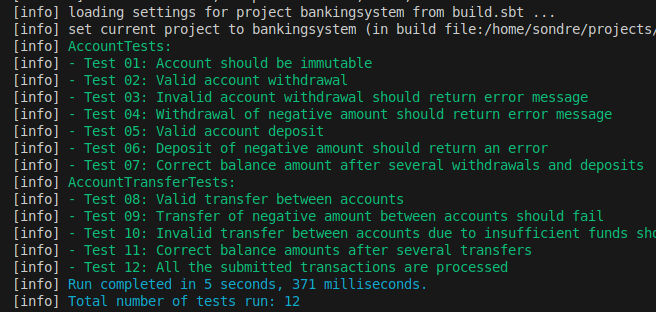
\includegraphics[width=\textwidth]{img/test.png}
  \caption{Tests}
\end{figure*}


\end{document}